\chapter{Physikalische Grundlagen}

1837 veröffentlichte der britische Mathematikprofessor \textsc{Charles Babbages} (1791-1871) den Entwurf einer Rechenmaschine namens \emph{Analytical Engine} (zu deutsch: Analytische Maschine).

\begin{figure}[htp]
\begin{center}%{r}{.6\textwidth}
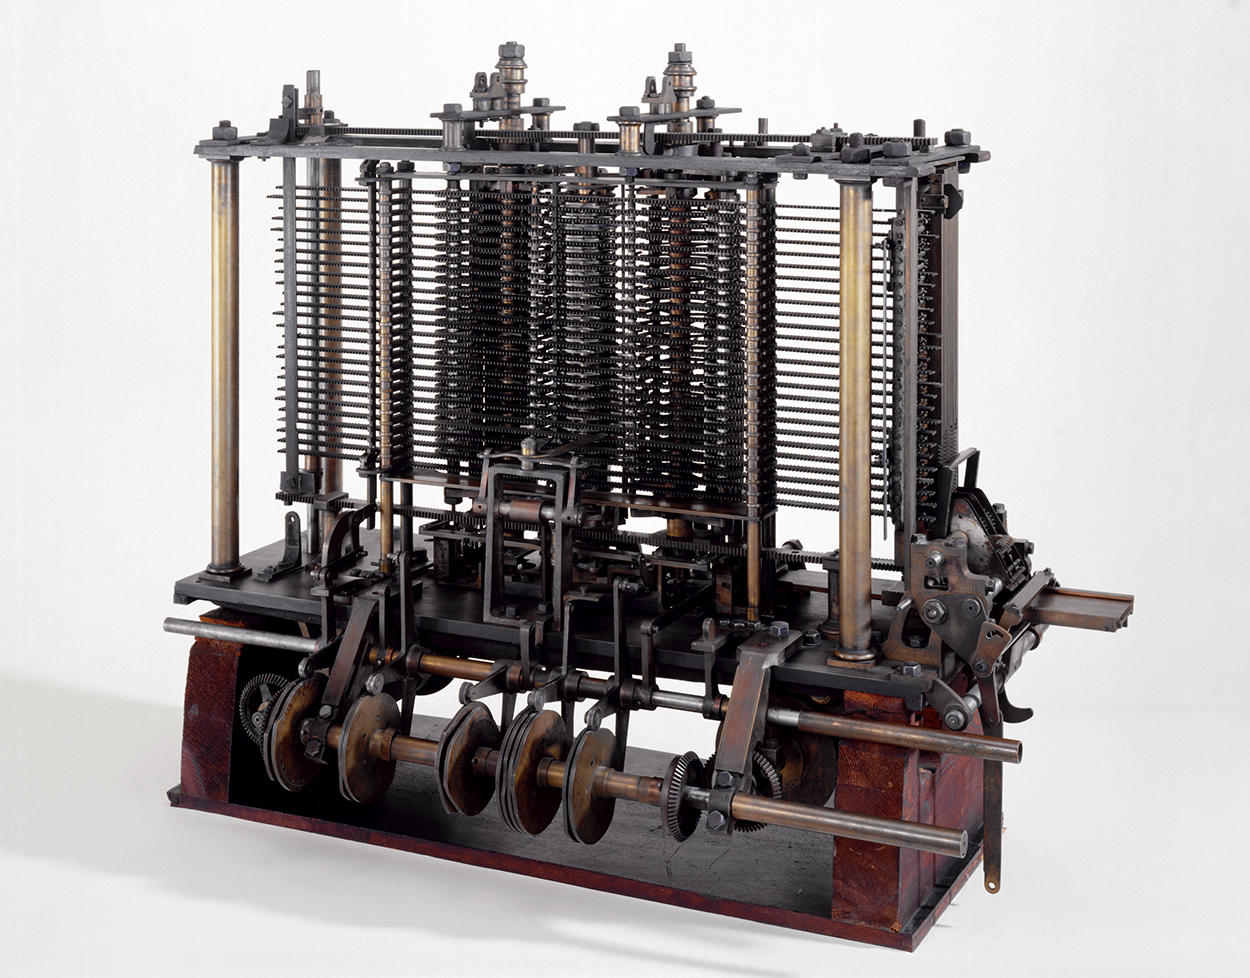
\includegraphics[scale=1.1]{pics/analyticengine}
\caption{Nachbau der \emph{Analytical Engine} (Quelle: wikipedia.org)}
\end{center}
\end{figure}


Dieser Entwurf gilt als wichtiger Schritt in der Geschichte der Entwicklung des Computers, denn hätte diese Maschine gebaut werden können, hätte man bereits einen frei programmierbaren Rechner gehabt, wie er erst ca. 100 Jahre später von dem deutschen Ingenieur \textsc{Konrad Zuse} erfunden wurde.

Diese Rechenmaschine arbeitete jedoch rein mechanisch.
Bei heutigen Computern kommt man an elektrischen Bauteilen und Halbleitern nicht vorbei.
Ohne Strom rechnet heute keine Maschine.
Doch was ist elektrischer Strom eigentlich?


\begin{Ziele}

In diesem Kapitel lernst du:

\begin{itemize}
\item Was ein Gleichstromkreis ist und welche wichtigen Größen dabei verwendet werden,
\item wie man das Programm \textsc{Yenka} benutzt, um Stromkreise zu simulieren,
\item welche wichtigen Gesetzmäßigkeiten in komplexeren Stromkreisen auftreten (die \textsc{Kirchhoff}schen Gesetze)
\item Welche wichtigen Stromkreise in einem Prozessor vorkommen (Logikgatter) und wie diese prinzipiell aufgebaut werden können.
\end{itemize}
\end{Ziele}


\section{Gesetze im Gleichstromkreis}

%\begin{code}
\begin{Aufgabe} \label{Aufg:Strom}
Überlege dir, wie man \emph{elektrischen Strom} physikalisch definieren kann.
Welche Rolle spielen dabei die Begriffe \emph{elektrischer Stromkreis} und \emph{Spannungsquelle}?
\end{Aufgabe}
%\end{code}


\begin{Loesung}[zu Aufgabe \ref{Aufg:Strom}]
Einige Lösungen findest du im Anhang zur Selbstkontrolle.
Wichtig ist, dass du dir die Lösungen erst ansiehst, nachdem du die Aufgabe bearbeitest hast, um einen Lernerfolg zu erzielen.

Die Lösung findest du in Lösung \ref{Loes:Strom}.
\end{Loesung}


Das Programm \textsc{Yenka} simuliert Stromkreise und Logikschaltungen am Computer.

%\begin{code}{1}
\begin{Aufgabe}
Befolge zunächst die folgenden Schritte:

\begin{itemize}
\item Öffne \textsc{Yenka} (zB. auf dem Desktop)!
\item Stelle die Spracheinstellung unten in der Mitte auf Englisch!
\item Wähle den Reiter \emph{Technologies} und in der Mitte links die Kategorie \emph{Electronics}!
\item Öffne eine neue Datei im Programm (links oben $\Rightarrow$ New)!
\item[(a)] Implementiere einen elektrischen Stromkreis, bestehend aus einer Batterie (Battery) und einer Lampe (Signal Lamp) (Electronic Components $\Rightarrow$ Basic Components $\Rightarrow$ Symbolic) und ändere den Spannungswert, indem du darauf klickst.
\item[(b)] Übernimm den Stromkreis als Zeichnung in dein Heft!
\item[\textcolor{red}{(ZA)}] Ergänze den Stromkreis durch einen Schalter (SPST) und vergleiche die Funktionsweise mit dem Stromkreis zuvor!
\end{itemize}
\end{Aufgabe}
%\end{code}


%\begin{code}{1}
\begin{Aufgabe}
\hfill \par \vspace*{-.8cm}
\begin{itemize}
\item[(a)] Benutze den letzten Stromkreis und miss die Stromstärke, indem du ein \emph{Amperemeter} (Lab Equipment $\Rightarrow$ Measurement) in den Stromkreis einfügst!
\item[(b)] Verändere den Spannungswert der Spannungsquelle! Beobachte die Veränderung am Amperemeter!
%\item[(c)] Formuliere den Zusammenhang zwischen Spannung und Stromstärke. 
%\item[\textcolor{red}{(ZA)}] Durch welche Größe hängen beide zusammen?
\end{itemize}
\end{Aufgabe}
%\end{code}


Du solltest bei der letzten Aufgabe beobachtet haben, dass mit höherer Spannung auch ein größerer Strom fließt (das \emph{Amperemeter} zeigt einen höheren Wert).
Bei näherer Betrachtung fällt sogar auf, dass die beiden Größen der Spannung und der Stromstärke proportional voneinander abhängen.

Die Proportionalitätskonstante nennt man den (elektrischen) Widerstand $R$.
Als Zusammenhang gilt demnach: $U = R \cdot I$ (das \textsc{Ohm}sche Gesetz).
Dabei ist $U$ die Spannung und $I$ die Stromstärke.

\begin{sich}[\textsc{Ohm}sches Gesetz]
$U = R \cdot I$ ($U$ - Spannung, $I$ - Stromstärke, $R$ - elektrischer Widerstand)

Der Wert der Spannung $U$ wird in Volt ($1V$) angegeben, der Wert der Stromstärke wird in Ampere ($1A$) angegeben. Der Wert des Widerstandes wird in Ohm ($1\Omega$) angegeben.
\end{sich}




%\begin{code}{1}
\begin{Aufgabe}
Füge in den letzten Stromkreis einen Widerstand ein (Electronic Components $\Rightarrow$ Basic Components $\Rightarrow$ Symbolic $\Rightarrow$ Resistor) und beobachte den Zusammenhang des Ohmschen Gesetzes, indem du die Spannungswerte veränderst.
\end{Aufgabe}
%\end{code}


%\begin{code}{1}
\begin{Aufgabe}
\hfill \par \vspace*{-.8cm}
\begin{itemize}
\item[(a)] Öffne im TI-Ordner (In die Adresszeile des Explorers (Dateiordner) eingeben: \textbackslash \textbackslash faust\textbackslash TI9) die Datei \emph{Knoten und Maschen.yka}
\item[(b)] Betrachte in der Schaltung oben die Stromstärken an den Amperemetern, während du die Widerstandswerte (durch darauf klicken) änderst!
Formuliere eine Beobachtung, wie die Stromstärken voneinander abhängen!
\item[(c)] Betrachte in der Schaltung unten die Spannungswerte an den Voltmetern, während du die Widerstandswerte änderst! 

Die Spannungswerte geben an, wie viel Spannung über dem jeweiligen Widerstand "'abfällt"'. Vom Pluspol der Spannungsquelle bis zum Minuspol muss die gesamte Spannung abfallen.
Formuliere eine Beobachtung, wie die Spannungswerte voneinander abhängen!
%\item[(c)] Formuliere schriftlich eine Vermutung, welche beiden Gesetzmäßigkeiten hier gelten. Teste deine Vermutung durch das Einstellen verschiedener Werte.
\end{itemize}
\end{Aufgabe}
%\end{code}




%% Erklärung der Kirchhoffschen Gesetze!

Die beiden Gesetzmäßigkeiten heißen \textsc{Kirchhoff}sche Gesetze (benannt nach dem preußisch/deutschen Physiker \textsc{Gustav Robert Kirchhoff}).

Diese können wie folgt formuliert werden:


\begin{sich}
\textbf{1. Kirchhoffsches Gesetz} (Knotensatz):


%\begin{wrapfigure}{r}{.55\textwidth}
%\begin{figure}[htp]
\begin{center}
%\begin{flushright}
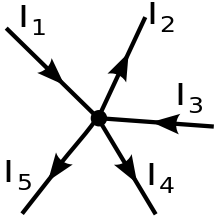
\includegraphics[scale=.8]{pics/knotenregel}
%\caption{Darstellung eines Knotens mit $I_1+I_3=I_2+I_4+I_5$ (Quelle: wikipedia.org)}
\captionof{figure}{Darstellung eines Knotens mit $I_1+I_3=I_2+I_4+I_5$ (Quelle: wikipedia.org)}
%\end{flushright}
\end{center}
%\end{figure}
%\end{wrapfigure}

Für jeden Knotenpunkt eines Netzwerkes gilt, dass die Summe der einfließenden Ströme gleich der Summe der herausfließenden Ströme ist.
\end{sich}

Alle Stromstärken addiert, die in einen Knotenpunkt fließen, müssen im gleichen Betrag also auch den Knotenpunkt wieder verlassen. Ähnlich wie bei zwei Flüssen, die zusammen fließen.

Für das zweite Kirchhoffsche Gesetz benötigen wir den Begriff der \emph{Masche}:

\begin{sich}
Eine \emph{Masche} ist ein geschlossener Kreis in einem Netzwerk.
Dieser Kreis muss keine Spannungsquelle besitzen.
\end{sich}

%\newpage
\begin{sich}
\textbf{2. Kirchhoffsches Gesetz} (Maschensatz):

%\begin{figure}[htp]
\begin{center}
%\begin{wrapfigure}{r}{.55\textwidth}
%\begin{flushright}
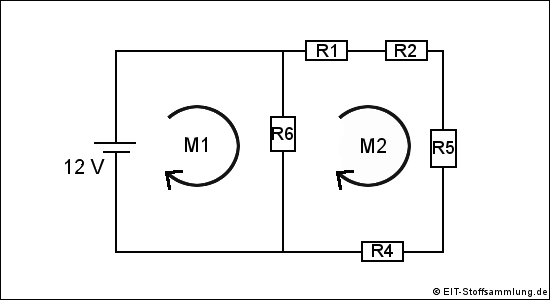
\includegraphics[scale=.8]{pics/maschensatz}
\captionof{figure}{Darstellung zweier Maschen (Quelle: eit-stoffsammlung.de)}
\label{Abb:Maschensatz}
%\end{flushright}
%\end{wrapfigure}
\end{center}
%\end{figure}

Die Spannungsabfälle über den Widerständen in jeder Masche eines Netzwerkes addieren sich zu null.
\end{sich}

Dabei legt man sich in einer Masche eine Drehrichtung fest.
Eine Spannung, die mit dieser Drehrichtung abfällt, wird positiv gewertet,
eine Spannung, die entgegen dieser Drehrichtung abfällt, wird negativ gewertet.
Addiert man so alle Spannungsabfälle, ergibt sich in jeder Masche stets 0.
Die Richtung eines Spannungsabfalls wird festgelegt durch den (technischen) Stromfluss (vom Plus- zum Minuspol), der über den Widerstand fließt.


\begin{Bsp}
In Abbildung \ref{Abb:Maschensatz} ist eine Masche durch $M1$ gegeben.
Als Drehrichtung wählen wir den Uhrzeigersinn.
Die Masche besteht aus der Spannungsquelle mit $U = 12~V$ und dem Widerstand $R_6$.

Der Spannungsabfall der Spannungsquelle ist $12~V$, da der gesamte Spannungswert vom Pluspol (oben) bis zum Minuspol (unten) abfallen muss.
Die Richtung des Spannungsabfalls ist somit von oben nach unten, also entgegen der festgelegten Drehrichtung.
Wir werten den Spannungsabfall damit negativ, also mit $-12~V$.

Die Spannung über $R_6$ fällt mit dem Drehsinn ab (der (technische) Stromfluss geht vom Plus- zum Minuspol der Spannungsquelle und damit von oben nach unten über $R_6$).
Damit werten wir $R_6$ positiv.

Es ergibt sich: $-12~V + U_6 = 0$, durch umstellen erhält man, dass der Spannungsabfall über $R_6$ ist: $U_6 = 12~V$.

In Masche $M2$ fällt die Spannung über $R_6$ negativ ab (entgegen der Drehrichtung), während alle weiteren Werte über $R_1, R_2, R_5$ und $R_4$ mit dem Drehsinn, also positiv abfallen.
Es ergibt sich: $-R_6 + R_1 + R_2 + R_5 + R_4 = 0$ (was ohne weitere Angaben nicht weiter berechnet werden kann).
\end{Bsp}


%\begin{code}{1}
\begin{Aufgabe} \label{Aufg:Kirchhoff1}
Ergänze die fehlenden Stromstärken, indem du die \textsc{Kirchhoff}schen Gesetze anwendest!

\begin{tabular}{cc}
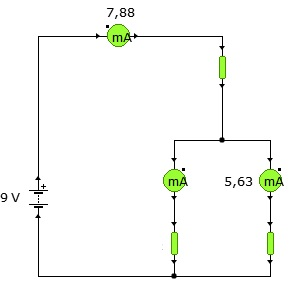
\includegraphics[scale=.9]{pics/Knoten1}
&
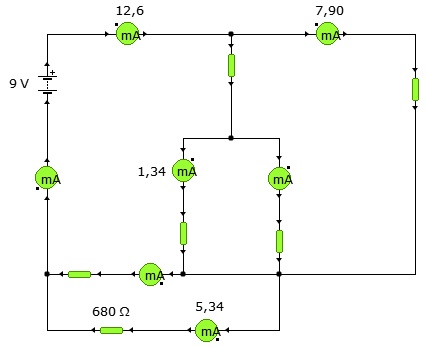
\includegraphics[scale=.7]{pics/Knoten2}
\\
(a) & (b)
\end{tabular}
\end{Aufgabe}
%\end{code}


%\begin{code}{1}
\begin{Aufgabe} \label{Aufg:Kirchhoff2}
Ergänze die fehlenden Spannungen, indem du die \textsc{Kirchhoff}schen Gesetze anwendest!

\begin{tabular}{cc}
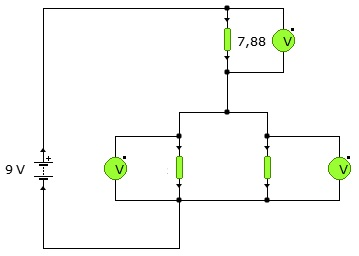
\includegraphics[scale=.8]{pics/Masche1}
&
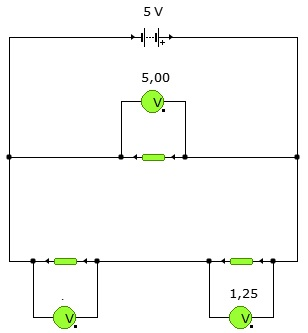
\includegraphics[scale=.8]{pics/Masche2}
\\
(a) & (b)
\end{tabular}
\centering
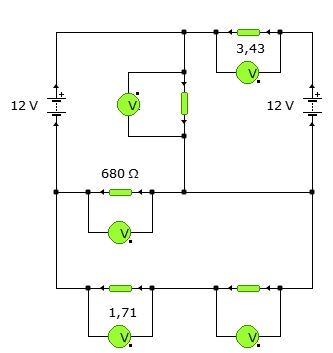
\includegraphics[scale=.9]{pics/Masche3}
\\
(c)
\end{Aufgabe}
%\end{code}



\section{Logikgatter} \label{Sec:Logikgatter}

Im Prozessor (CPU) eines Computers kommen Gleichstromkreise als sogenannte \emph{Logikgatter} oder \emph{Logische Schaltungen} vor.
Diese implementieren logische Grundfunktionen aus der Mathematik.


%\begin{code}{1}
\begin{Aufgabe}
Teste die folgenden Logikgatter in \textsc{Yenka} (Electronic Components $\Rightarrow$ Digital Processing $\Rightarrow$ Digital 4000 Series $\Rightarrow$ Logik Gates) implementiere dazu neben den Gattern auch Schalter als Eingänge (Lab Equipment $\Rightarrow$ Logic $\Rightarrow$ Latching Logic Input) und einen Ausgang (Logic Indicator im selben Ordner).

Fülle die Schalttabellen entsprechend aus und übernimm dir das Schaltsymbol und den logischen Term in dein Heft!

\vspace*{.7cm}

\textbf{AND-Gatter}

\begin{tabular}{ll}
Schalttabelle:~~~~~~~~~~~~~~~~~~ & Schaltsymbol: \\
\begin{tabular}{|c|c||c|}
\hline
$a$ & $b$ & $A$~~ \\ \hline \hline
0 & 0 &  \\ 
0 & 1 &  \\
1 & 0 &  \\
1 & 1 &  \\ \hline
\end{tabular}
&
\begin{minipage}{.6\textwidth}
\begin{center}
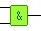
\includegraphics[scale=1.5]{pics/AND.jpg}
\end{center}

Logischer Term: \\
\begin{align*}
A = a \wedge b
\end{align*}
\end{minipage}

\end{tabular}




\textbf{OR-Gatter}

\begin{tabular}{ll}
Schalttabelle:~~~~~~~~~~~~~~~~~~ & Schaltsymbol: \\
\begin{tabular}{|c|c||c|}
\hline
$a$ & $b$ & $A$~~ \\ \hline \hline
0 & 0 &  \\ 
0 & 1 &  \\
1 & 0 &  \\
1 & 1 &  \\ \hline
\end{tabular}
&
\begin{minipage}{.6\textwidth}
\begin{center}
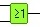
\includegraphics[scale=1.5]{pics/OR.jpg}
\end{center}

Logischer Term: \\
\begin{align*}
A = a \vee b
\end{align*}
\end{minipage}

\end{tabular}




\textbf{NOT-Gatter}

\begin{tabular}{ll}
Schalttabelle:~~~~~~~~~~~~~~~~~~ & Schaltsymbol: \\
\begin{tabular}{|c||c|}
\hline
$a$ & $A$~~ \\ \hline \hline
0 &   \\ 
1 &   \\ \hline
\end{tabular}
&
\begin{minipage}{.6\textwidth}
\begin{center}
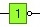
\includegraphics[scale=1.5]{pics/NOT.jpg}
\end{center}

Logischer Term: \\
\begin{align*}
A = \neg a 
\end{align*}
\end{minipage}

\end{tabular}
\end{Aufgabe}
%\end{code}

%\begin{code}{1}
\begin{Aufgabe}
Implementiere in \textsc{Yenka} je Logikgatter einen Gleichstromkreis, der das jeweilige Gatter simuliert. Die Eingänge sollen dabei durch Kippschalter realisiert werden. Als Ausgang soll eine Lampe oder LED dienen.
\begin{itemize}
\item[\textcolor{red}{(ZA)}] Implementiere auf gleiche Weise die Kombinationen $\neg (a \wedge b)$ und \\ $\neg (a \vee b)$!
\end{itemize}
\end{Aufgabe}
%\end{code}

Im Prozessor kommen Schaltungen natürlich nicht mit mechanischen Schaltern daher.
Beim "'Schalten"' im Prozessor handelt es sich um elektronisch gesteuerte Prozesse, da diese automatisiert werden können.

Wie das elektronische schalten funktioniert, klärt das nächste Kapitel.


\section*{Zusammenfassung}

In diesem Kapitel hast du gelernt...

\begin{itemize}
\item dass für einen Stromfluss ein Stromkreis mit einer Spannungsquelle benötigt wird,
\item dass die Größen der Spannung $U$, der Stromstärke $I$ und des (elektrischen) Widerstands $R$ im Gleichstromkreis wichtig sind und durch das \textsc{Ohm}sche Gesetz folgendermaßen in Zusammenhang stehen: $U = R \cdot I$,
\item dass der Betrag der Stromstärken, die in einen Knotenpunkt eines Netzwerkes zusammenfließen im selben Betrag aus diesem auch herausfließen (1. \textsc{Kirchhoff}sches Gesetz),
\item dass sich die Spannungsabfälle über den Widerständen einer Masche stets zu null addieren (2. \textsc{Kirchhoff}sches Gesetz) und
\item dass in einem Computer die Logikgatter AND, OR und NOT vorkommen und diese mit Hilfe eines Gleichstromkreises und Schaltern simuliert werden können.
\end{itemize}